\documentclass[a4paper,oneside,DIV=10,12pt]{scrartcl}

\usepackage{graphicx}
\usepackage{float}

\usepackage{fontspec}
\setmainfont{STIX Two Text}
%\setsansfont{Roboto}
\newfontfamily{\cyrillicfontsf}{Roboto}

\usepackage{microtype}

\usepackage{polyglossia}
\setmainlanguage{ukrainian}

\usepackage{amsmath}
\usepackage{unicode-math}
\setmathfont{STIX Two Math}

\usepackage{booktabs}

\usepackage{tikz}
\usetikzlibrary{arrows,automata,positioning}

\usepackage{siunitx}
\sisetup{output-decimal-marker = {,},
exponent-product = {\cdot}}

% Problem-solution typesetting
\usepackage{xsim}
\DeclareExerciseTranslations{exercise}{
	Ukrainian	=	завдання ,
}

\DeclareExerciseTranslations{solution}{
	Ukrainian	=	розв'язання ,
}

\xsimsetup{
	solution/print = true,
}

\renewcommand{\implies}{\rightarrow}

\newcommand\barneg[1]{\overline{#1}}

\begin{document}
	\begin{titlepage}
		\begin{center}
			Міністерство освіти і науки України\\
			Національний авіаційний університет\\
			Навчально-науковий інститут комп'ютерних інформаційних технологій\\
			Кафедра комп'ютеризованих систем управління
			
			\vspace{\fill}
				Академічна різниця\\
				з дисципліни:\\
				«Комп'ютерна логіка»\\
				I семестр
				
			\vspace{\fill}
			
			\begin{flushright}
				Виконав:\\
				студент ННІКІТ СП-225\\
				Клокун Владислав\\
			\end{flushright}
			Київ 2017
		\end{center}
	\end{titlepage}
	
	\begin{exercise}
		Опишіть логічні (булеві) функції від двох змінних.
	\end{exercise}
	
	\begin{solution}	
		Булева функція від двох змінних --- це відображення $B^2 \mapsto B$, де $B = \{0, 1\}$. Для двох аргументів всього існує $2^{2^2} = 16$ можливих булевих функцій. 
	\end{solution}
	
	\begin{exercise}
		Побудувати таблицю істинності для функції
		\[
			F(x, y, z) = \left( \barneg{xy} \implies z\right) \left( x \barneg{z} \implies y \right).
		\]
	\end{exercise}
	
	\begin{exercise}
		Виконайте спрощення логічного виразу
		\[
			L = X_3X_2 \lor X_3 \barneg{X_2} \lor \barneg{\barneg{X_1} \lor \barneg{X_1 \lor X_2} }.
		\]
		Виконайте мінімізацію логічного виразу
		\[
			F = 0 \lor 4 \lor 7 \lor 8 \lor 11 \lor\ 12 \lor 13 \lor 15.
		\]
	\end{exercise}
	
	\begin{exercise}
		Отримати МДНФ перемикальних функцій, що задані діаграмами Вейча.
		
		\begin{figure}[!htbp]
		\centering
			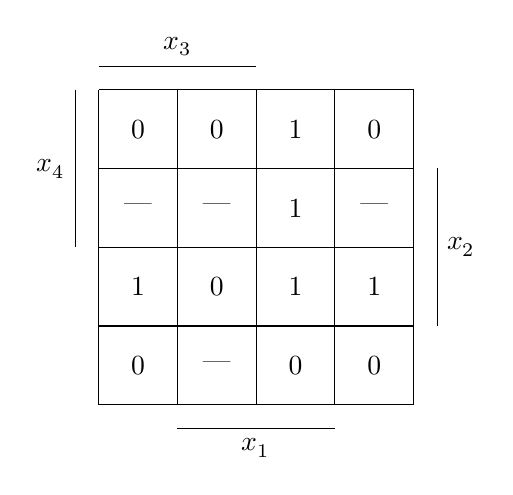
\begin{tikzpicture}
				\draw (0,0) grid (4,4);
				\node at (0.5,0.5){0};
				\node at (1.5,0.5){—};
				\node at (2.5,0.5){0};
				\node at (3.5,0.5){0};

				\node at (0.5,1.5){1};
				\node at (1.5,1.5){0};
				\node at (2.5,1.5){1};
				\node at (3.5,1.5){1};
				
				\node at (0.5,2.5){—};
				\node at (1.5,2.5){—};
				\node at (2.5,2.5){1};
				\node at (3.5,2.5){—};
				
				\node at (0.5,3.5){0};
				\node at (1.5,3.5){0};
				\node at (2.5,3.5){1};
				\node at (3.5,3.5){0};
				
				\draw (0,4.3) --node[midway, above]{$x_3$} (2,4.3);
				\draw (-0.3,4) --node[midway, left]{$x_4$} (-0.3,2);
				\draw (1,-0.3) --node[midway, below]{$x_1$} (3,-0.3);
				\draw (4.3,1) --node[midway, right]{$x_2$} (4.3,3);
			\end{tikzpicture}
		\end{figure}
		
		Для мінімізації застосувати метод Квайна~--- МакКласкі. Перемикальну функцію реалізувати в елементному базисі АБО---НЕ.
	\end{exercise}
	
	\begin{exercise}
		За даним графом автомата виконати синтез керуючого автомата.
		
		\begin{figure}[!htbp]
		\centering
			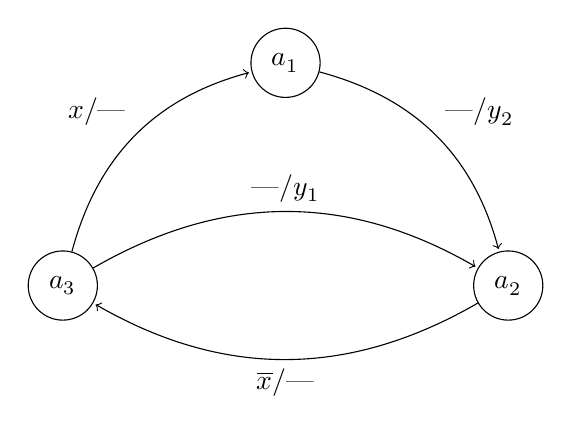
\begin{tikzpicture}[shorten >=1pt,node distance=4cm,on grid,auto]
				
				\node[state]	(a_1)		{$a_1$};
				\node[state]	(a_2) [below right=of a_1]	{$a_2$};
				\node[state]	(a_3) [below left=of a_1]	{$a_3$};
				
				\path[->]	(a_1)	edge [bend left=30]	node {$— / y_2$}	(a_2)
							(a_2)	edge [bend left=30]	node {$\barneg{x} / —$}				(a_3)
							(a_3)	edge [bend left=30]	node {$x / —$}		(a_1)
									edge [bend left=30]	node {$— / y_1$}	(a_2);
				
			\end{tikzpicture}
		\end{figure}
		Для побудови функціональної схеми використати T-тригери. Елементний базис: І, АБО, НЕ.
	\end{exercise}
\end{document}